\documentclass{ee208report}

\title{Lab Report 11}

\begin{document}

\begin{CJK}{UTF8}{gbsn}
    \maketitle
\end{CJK}

\begin{multicols*}{2}

\section{Introduction}

In this lab report, we present our implementation of the Canny edge detector,
whose ideas are first proposed by, as the name suggests, John F. Canny in 1986.
The Canny edge detector is the most used edge detectors.

The report is organized as follows: A brief review of the Canny edge detector is
given in the next section. Then, an implementation of the Canny edge detector in
Python is introduced. There is also a section dedicated to threshold selection.
Finally, we conclude our report by comparing our implementation with that of
OpenCV, which is implemented in C++ and can interact with Python.

\section{Process of Edge Detection}

The process of edge detection can be broken down into 5 steps:

\begin{description}
    \item[Filtering] Apply Gaussian filtering to the image to remove noises.
    \item[Finding gradients] Find the intensity gradients.
    \item[Non-maximum suppression] Thin the edges by suppressing gradients that
    are not local maximum.
    \item[Double thresholds] Mark pixels with gradients greater than the higher
    threshold (``strong edges'') as edges in the output image
    \item[Tracking edges by hysteresis] Mark pixels with gradients between the
    lower and higher threshold (``weak edges'') as edges only if there is a
    strong edge in its $3 \times 3$ neighborhood.
\end{description}

\section{Implementation}

\subsection{Filtering and Gradients}

OpenCV's built-in \texttt{Sobel()} function combines the Gaussian filtering with
applying the Sobel operators to the image to find the x- and y-derivatives. The
derivatives are later used to find the magnitudes and angles of gradients.

\begin{minted}[frame=lines]{python}
# find the gradients in x and y directions
dx = cv.Sobel(img, cv.CV_32F, 1, 0)
dy = cv.Sobel(img, cv.CV_32F, 0, 1)
# magnitudes of gradients and tangents of
# angles
mag = np.sqrt(dx * dx + dy * dy)
tangents = dy / (dx + 1e-6)
\end{minted}

The output type of the derivatives is set to \texttt{cv.CV\_32F} i.e. 32-bit
floats to preserve precision. After the gradients are calculated, a mesh
(Figure~\ref{fig:mesh-gradient}) is drawn about the magnitudes of gradients.

\begin{minted}[frame=lines]{python}
# draw a mesh about gradients
plt.contourf(np.flip(mag, 0))
plt.colorbar()
plt.savefig('canny_output/1_gradient_mesh.png')
plt.close()
\end{minted}

\begin{figure}[H]
    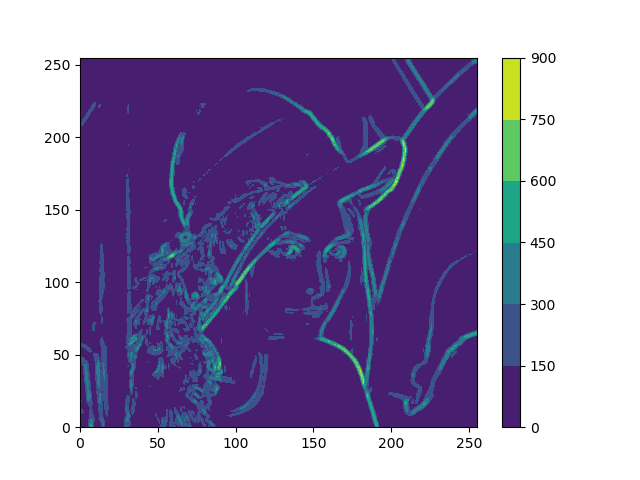
\includegraphics[width=\linewidth]{images/1_gradient_mesh.png}
    \caption{A mesh plot about the magnitudes of gradients}
    \label{fig:mesh-gradient}
\end{figure}

\subsection{Non-maximum suppression}

Non-maximum is an edge-thinning technique. It is evident from the mesh plot in
Figure~\ref{fig:mesh-gradient} that sudden increase in gradients almost always
occur in groups of pixels rather than individual pixels. The idea of
non-maximum suppression is simple: in a group of pixels with a sudden increase
in gradient magnitude that may be attributed to the same edge, for each pixel,
compare its gradient magnitude with other gradients in its gradient direction.
A gradient will be suppressed if it is less than either of the two gradients.

For a $3 \times 3$ neighborhood of the pixel $(i, j)$, if the gradient of
$(i, j)$ does not fall into one of the eight directions (north, south, east,
west, northwest, northeast, southwest, southeast), we have to interpolate two
gradients from neighboring gradients. Figure~\ref{fig:neighborhood} illustrates
one possible case:

\begin{figure}[H]
    \includegraphics[width=\linewidth]{image_representation.pdf}
    \caption{$3 \times 3$ neighborhood showing how gradient interpolation works}
    \label{fig:neighborhood}
\end{figure}

The gradient direction is indicated by the line crossing the origin. Gradient
magnitudes between $(i + 1, j + 1)$, $(i, j + 1)$ and $(i, j - 1)$,
$(i - 1, j - 1)$ must be interpolated. For example, to interpolate the gradient
in the first quadrant in Figure~\ref{fig:neighborhood}, we simply write

\[
    v = \textrm{ mag}[i][j + 1] \tan \theta + \textrm{ mag}[i + 1][j + 1] (1 -
    \tan \theta)
\]

where $v$ is the new magnitude of gradient. Figure~\ref{fig:neighborhood} also
forms the basis for our implementation in Listing~\ref{lst:non-max-sup} in the
appendix. Again, we draw a mesh in Figure~\ref{fig:post-suppression-mesh} of
gradients after suppression. Compared with Figure~\ref{fig:mesh-gradient}, the
edges have shrunk considerably.

\begin{figure}[H]
    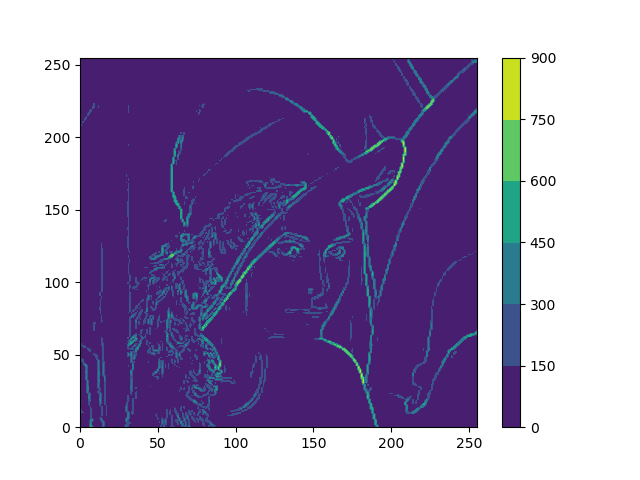
\includegraphics[width=\linewidth]{images%
/1_gradient_mesh_post_suppression.png}
    \caption{Mesh plot for post-suppression gradients}
    \label{fig:post-suppression-mesh}
\end{figure}

\subsection{Double thresholds}

To mark strong edges in the output image, we write

\begin{minted}[frame=lines]{python}
# init the image for output
edges = np.zeros(img.shape, np.uint8)
# double thresholds
# mark strong edges as white in the output
edges[mag >= t2] = 255
cv.imwrite('canny_output/1_2t.png', edges)
\end{minted}

The edges at this stage is shown in Figure~\ref{fig:strong-edges}.

\begin{figure}[H]
    \centering
    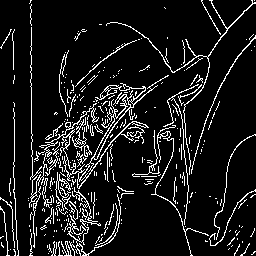
\includegraphics[width=0.8\linewidth]{images/1_2t.png}
    \caption{Strong edges in the image after thresholding}
    \label{fig:strong-edges}
\end{figure}

\subsection{Tracking edges}

Basically, a weak edge is preserved if there is a strong edge in its
$3 \times 3$ neighborhood. Implementation is available in
Listing~\ref{lst:edge-tracking}. Figure~\ref{fig:output-edges} shows the final
output.

\begin{figure}[H]
    \centering
    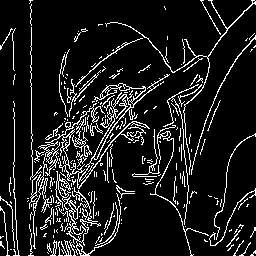
\includegraphics[width=0.8\linewidth]{images/1_final.png}
    \caption{Output edges}
    \label{fig:output-edges}
\end{figure}

Edges detected in \texttt{2.jpg} and \texttt{3.jpg} are available in
Figure~\ref{fig:other-edges} and in \texttt{2\_final.png} and
\texttt{3\_final.png}.

\begin{figure}[H]
    \centering
    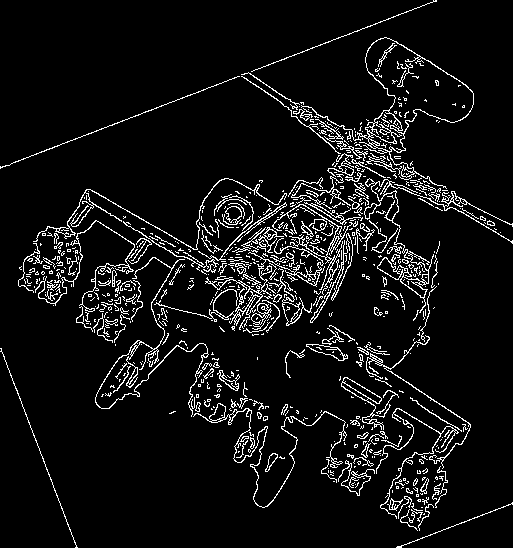
\includegraphics[width=\linewidth]{images/2_final.png}
    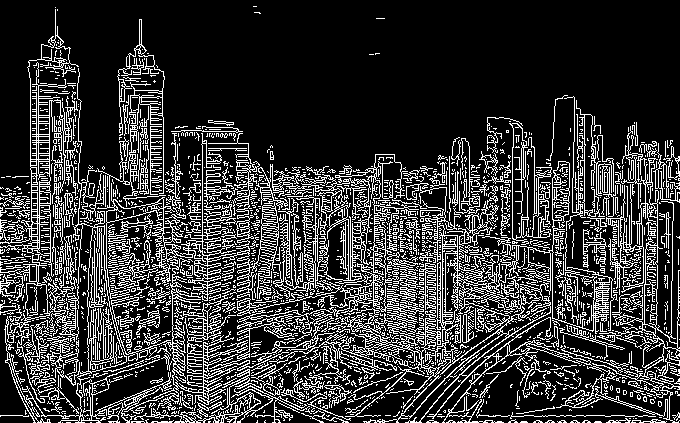
\includegraphics[width=\linewidth]{images/3_final.png}
    \caption{Edges for \texttt{2.jpg} and \texttt{3.jpg}}
    \label{fig:other-edges}
\end{figure}

\section{Thresholds Selection}

We write a simple Python script, \texttt{test\_thresholds.py}, that selects a
wide range of thresholds and generates output images for each pair of
thresholds. Figure~\ref{fig:high-t} shows 6 images of edges processed with a
high threshold between 60 and 110 (inclusive).\footnote{We would advise readers
to view these images in image viewer software rather than in the paper, because
flipping through the images give a better idea of how the noises change with
different thresholds. These images are located under the
\texttt{high\_threshold} and \texttt{low\_threshold} folders} There is a sharp
increase of noises when the high threshold transitions from 80 to 70 and then 60
, while increasing the threshold from 80 upwards does nothing more than removing
edges.

Figure~\ref{fig:low-t} shows 6 images with varying low thresholds. But different
thresholds doesn't have significant influence over the final image and only add
minute details.

\section{Time Comparison}

We select the 40 as the low threshold and 100 as the high threshold. Each
function runs on each image for 100 times with \texttt{timeit.timeit()}.
All time refers to a single execution of the function.

\begin{table}[H]
\begin{tabular}{lrr}
    \toprule
    Image & Handcrafted \texttt{canny()}/s & \texttt{cv.canny()}/s \\
    \midrule
    \texttt{1.jpg} & 1.4933 & 0.005938 \\
    \texttt{2.jpg} & 5.5464 & 0.001110 \\
    \texttt{3.jpg} & 5.5330 & 0.001646 \\
    \bottomrule
\end{tabular}
\caption{Running time cross-comparison}
\label{tbl:time}
\end{table}

As Table~\ref{tbl:time} shows, the built-in function \texttt{cv.canny()} runs
almost 500 times faster than our handcrafted version in the best case.

\section{Conclusion}

The Canny edge detector, although simple in its implementation, turns out to
work extraordinarily well.

\end{multicols*}

\begin{figure}[H]
    \centering
    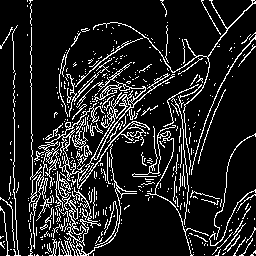
\includegraphics[width=0.35\linewidth]{images/high_threshold/60.png}
    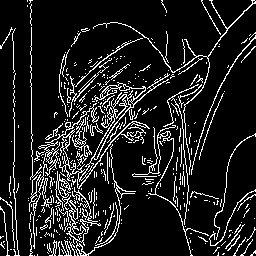
\includegraphics[width=0.35\linewidth]{images/high_threshold/70.png}
    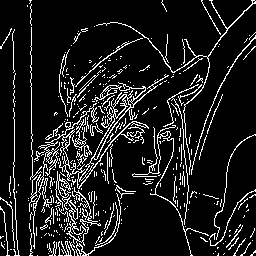
\includegraphics[width=0.35\linewidth]{images/high_threshold/80.png}
    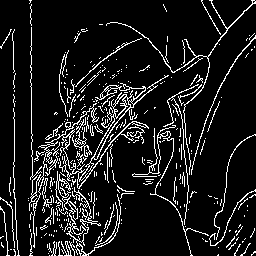
\includegraphics[width=0.35\linewidth]{images/high_threshold/90.png}
    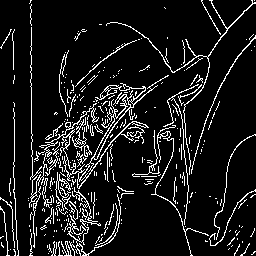
\includegraphics[width=0.35\linewidth]{images/high_threshold/100.png}
    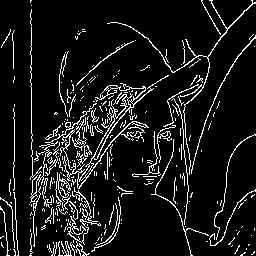
\includegraphics[width=0.35\linewidth]{images/high_threshold/110.png}
    \caption{6 images after non-maximum suppression but before edge tracking.
    The thresholds for each image increases by 10 in a left-to-right, top down
    manner. The upper left image has a high threshold of 60 and the lower right
    has 110.}
    \label{fig:high-t}
\end{figure}

\begin{figure}[H]
    \centering
    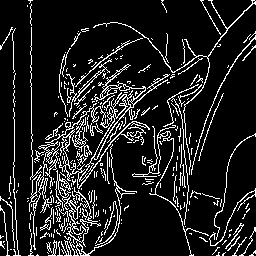
\includegraphics[width=0.35\linewidth]{images/low_threshold/20.png}
    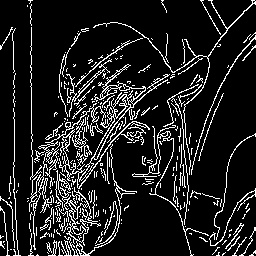
\includegraphics[width=0.35\linewidth]{images/low_threshold/30.png}
    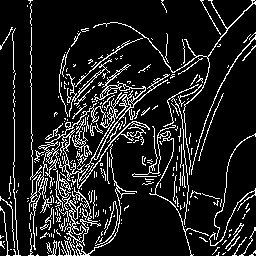
\includegraphics[width=0.35\linewidth]{images/low_threshold/40.png}
    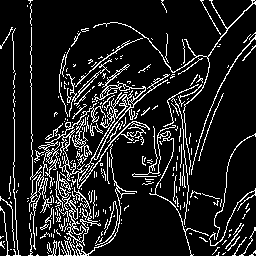
\includegraphics[width=0.35\linewidth]{images/low_threshold/50.png}
    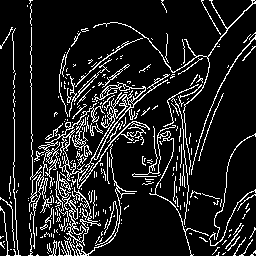
\includegraphics[width=0.35\linewidth]{images/low_threshold/60.png}
    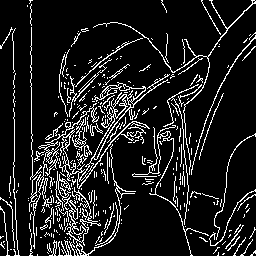
\includegraphics[width=0.35\linewidth]{images/low_threshold/70.png}
    \caption{6 images after edge tracking. Each image has a high threshold of
    80. The low thresholds for each image increases by 10 in a left-to-right,
    top down manner. The upper left image has a low threshold of 20 and the
    lower right has 70.}
    \label{fig:low-t}
\end{figure}

\begin{listing}
    \begin{minted}[linenos, frame=lines]{python}
for i in range(1, mag.shape[0] - 1):
    for j in range(1, mag.shape[1] - 1):
        if tangents[i][j] >= 1:
            cot = 1 / tangents[i][j]
            # Interpolate the upper gradient. "Upper" means the direction
            # in which y is increasing.
            mag_upper = mag[i + 1][j] * (1 - cot) + mag[i + 1][j + 1] * cot
            # interpolate the lower gradient
            mag_lower = mag[i - 1][j] * (1 - cot) + mag[i - 1][j - 1] * cot
        elif tangents[i][j] >= 0:
            mag_upper = mag[i][j + 1] * (1 - tangents[i][j]) + mag[i + 1][j + 1] * tangents[i][j]
            mag_lower = mag[i][j - 1] * (1 - tangents[i][j]) + mag[i - 1][j - 1] * tangents[i][j]
        elif tangents[i][j] >= -1:
            mag_upper = mag[i][j - 1] * (1 + tangents[i][j]) - mag[i + 1][j - 1] * tangents[i][j]
            mag_lower = mag[i][j + 1] * (1 + tangents[i][j]) - mag[i - 1][j + 1] * tangents[i][j]
        else:
            cot = 1 / tangents[i][j]
            mag_upper = mag[i + 1][j] * (1 + cot) - mag[i + 1][j - 1] * cot
            mag_lower = mag[i - 1][j] * (1 + cot) - mag[i - 1][j + 1] * cot

        # intensity at (i, j) is not greater than its neighbors
        if mag[i][j] <= mag_lower or mag[i][j] <= mag_upper:
        suppressed_mag[i][j] = 0
    \end{minted}
    \caption{Implementation of non-maximum suppression}
    \label{lst:non-max-sup}
\end{listing}

\begin{listing}
    \begin{minted}[linenos, frame=lines]{python}
# index offsets for 8 cases:
# -1, -1    -1, 0   -1, 1
# 0, -1     0, 0    0, 1
# 1, -1     1, 0    1, 1
OFFSETS = np.array(((-1, -1), (-1, 0), (-1, 1), (0, -1), (0, 1), (1, -1),
(1, 0), (1, 1)), np.int8)
# hysteresis
for i in range(img.shape[0]):
    for j in range(img.shape[1]):
        if t1 <= mag[i][j] < t2:    # if this is a weak edge
            for offset_i, offset_j in OFFSETS:
                i_ = i + offset_i
                j_ = j + offset_j
                # if the index pair (i_, j_) is within the image border
                if 0 <= i_ < img.shape[0] and 0 <= j_ < img.shape[1]:
                    if mag[i_][j_] >= t2:
                        edges[i][j] = 255   # mark weak edges
                        break
    \end{minted}
    \caption{Implementation of edge tracking}
    \label{lst:edge-tracking}
\end{listing}

\end{document}
